\chapter{Planificación}

\section{Historias de usuario}

Se ha abordado la planificación del proyecto siguiendo metodologías ágiles, con historias de usuario definiendo la funcionalidad necesaria a implementar desde el punto de vista del usuario, y además, iterando sobre las tareas desde implementaciones básicas, pero funcionales, hasta conformar las más complejas y completas. \\ 

Se ha planificado el desarrollo en tres grandes hitos:

\begin{enumerate}
	\item \textbf{Servicio de mensajería}
	\item \textbf{Uso del protocolo Signal}
	\item \textbf{Despliegue de la aplicación en la red TOR}
\end{enumerate}

Se han conseguido realizar únicamente dos de tres de estos hitos planteados inicialmente; el último de ellos no ha sido completado pero se ha realizado una investigación referente a la tecnología, el funcionamiento y las posibilidades de implementación de la solución al hito. \\ 

A continuación se detallan, agrupadas por hitos, las distintas tareas realizadas: \\ 


\subsection{Hito 1: Sistema de mensajería}
\begin{adjustbox}{margin=2.5ex 5ex 2.5ex 2.5ex,center}
	\begin{forest} for tree={
	    growth parent anchor=south,
	    parent anchor=south,
	    child anchor=north,
	    edge path={none}, 
	    l sep=.25cm,
	}   
	%
	[Sistema de mensajería, goal, name=agoal
	    [Cliente, activity
	        [1. Conexión básica con el servidor, task
	       	[2. Mostrar mensaje de bienvenida{,} logo y login, task
	        [3. Mostrar usuarios conectados, task
	        [4. Iniciar conversación con un usuario, task
			[5. Mostrar usuario en la barra de navegación durante conversación, task
			[6. Recibir mensajes enviados al usuario cuando éste se encuentra desconectado, task			
	        [7. Link para volver a la lista de usuarios desde la conversación, task
	        [8. Actualizar estado de usuarios en tiempo real cuando estos se conectan/desconectan, task
	        [9. Mejora de estilos de vista\, presentación y efectos visuales, task	        
	        [9. Conectar con servidor desplegado, task	  	        
	        ] ] ] ] ] ] ] ] ] ] ]
	    [Servidor, activity
	        [1. Conexión básica con los clientes, task
			[2. Permitir registro de usuarios en la aplicación mediante nombre, task
	        [3. Enviar información respecto a usuarios conectados a los clientes, task
	        [4. Redirigir mensajes entre clientes en las conversaciones, task
	        [5. Almacenar mensajes cuando los usuarios están desconectados\, enviarlos cuando se conectan, task
	        [6. Enviar actualizaciones de usuarios conectados/desconectados en tiempo real a los clientes, task
 	        [6. Desplegar en una máquina servidor, task
	        ] ] ] ] ] ] ] ] ]
	%           
	\end{forest}
\end{adjustbox}

Una vez alcanzado este hito, la funcionalidad del proyecto cubre las necesidades básicas para mantener un sistema de chat entre múltiples usuarios en tiempo real. Esto supone la base sobre la que se implementarán las medidas de cifrado y seguridad.
	
\subsection{Hito 2: Uso del protocolo Signal}

\begin{adjustbox}{margin=2.5ex 5ex 2.5ex 2.5ex,center}
	\begin{forest} for tree={
			growth parent anchor=south,
			parent anchor=south,
			child anchor=north,
			edge path={none}, 
			l sep=.25cm,
	}   
	%
	[Uso del protocolo Signal, goal, name=bgoal
		[Cliente, activity
		[1. Generación de claves de cifrado al iniciar la aplicación, task
		[2. Solicitar y proveer claves al servidor según sea necesario durante la conversación, task
		[3. Cargar sesión con el usuario con el que se desee establecer una conversación, task
		[4. Descifrar mensajes entrantes usando claves de cifrado del usuario con el que se conversa, task
		[5. Cifrar mensajes al enviarlos{,} en el formato adecuado, task] ] ] ] ] ]
		[Servidor, activity
		[1. Redirigir peticiones y respuestas a peticiones de claves, task] ] ] 
	%           
	\end{forest}
\end{adjustbox}

En este hito se ha pretendido implementar la funcionalidad básica de cifrado del protocolo Signal, generando claves para cada mensaje intercambiado. \\

Una nueva clave publica es derivada de la clave privada de los usuarios a cada mensaje que se desea enviar, y se comprueba la validez de los mensajes mediante la firma de los mismos con la clave de identidad de cada usuario.
El servidor se trata finalmente como una entidad en la que no se confía, y la información que pasa a través del mismo no es accesible en texto plano. \\

Una vez implementado este punto, damos por implementada la funcionalidad que trata de preservar la privacidad en la comunicación. \\ 

\subsection{Hito 3: Despliegue en la red Tor}
\begin{adjustbox}{margin=2.5ex 5ex 2.5ex 2.5ex,center}
	\begin{forest} for tree={
			growth parent anchor=south,
			parent anchor=south,
			child anchor=north,
			edge path={none}, 
			l sep=.25cm,
	}   
	%
	[Despliegue en la red Tor, goal, name=cgoal
		[Cliente, activity
		[Conectar al servidor mediante la red TOR, task] ]
		[Servidor, activity
		[Deplegar servidor como hidden service, task
		[Conectar clientes a través de la red TOR, task ] ] ] ] 
	%           
	\end{forest}
\end{adjustbox}

En este hito se pretende cubrir el aspecto de la protección de la identidad de los usuarios, mediante la conexión a través de la red TOR. Así como de la ofuscación del servidor, desplegándolo como hidden service \cite{HiddenServiceTorProject} en la misma red. \\

\section{Diagrama de componentes}

\begin{figure}[H]
	\centering
	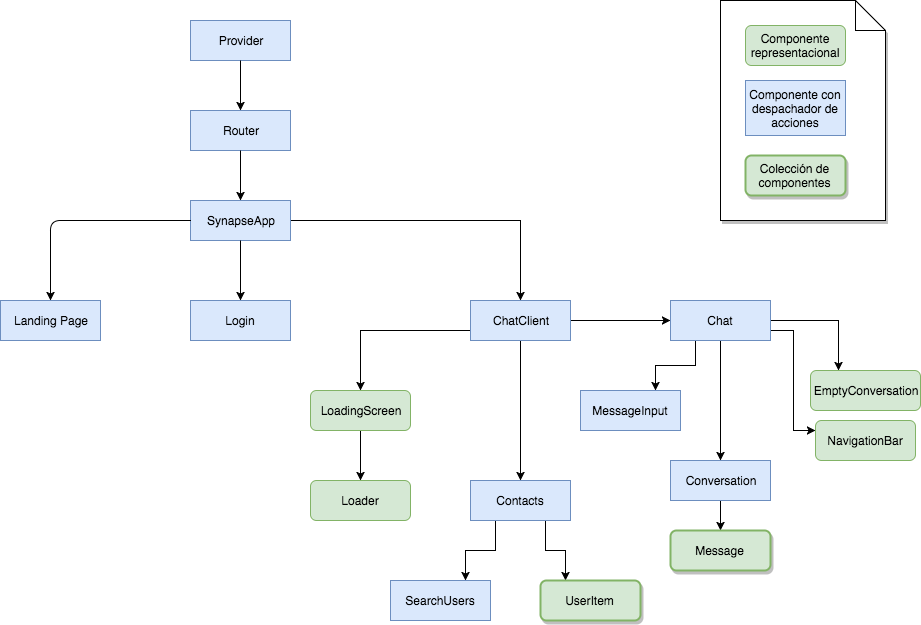
\includegraphics[width=\textwidth]{imagenes/diagrama-componentes}
	\caption{Diagrama de componentes}
	\label{fig:diagrama-componentes}
\end{figure}

Las aplicaciones React se estructuran en componentes ordenados en una jerarquía padre-hijo, donde los hijos reciben propiedades (props) del padre, y notifican a este de cambios en el estado según la interacción del usuario a través de llamadas a funciones, también recibidas por el mismo mecanismo que las propiedades.\\ 

Debido a esta naturaleza de React no se ha realizado un diagrama de clases UML. Sino que se ha realizado un diagrama donde se representan estas relaciones padre-hijo entre componentes y se hace distinción entre aquellos puramente representacionales (sin lógica) y aquellos que despachan acciones. \\ 